\section{Development}

When trying to follow a traditional software engineering approach to in
Haskell, one soon runs into several dead ends: due to the different paradigm
and style, trying to apply some methods feels forced or unnatural.
Traditionally, in Haskell the approach when formalizing a piece of code just
involves a mathematical validation, using pure Mathematics for a formal design
through equations, that can then verified by a theorem prover such as Agda or
Coq. Furthermore, the problems only increase when we try to use UML: this
methodology was clearly not designed for other than Object-Oriented programming
and it is not possible to create traditional diagrams for Haskell without
running in unforgivable simplifications, inaccuracies regarding the system or
simply nonsensical diagrams. \\

However, due to the academic character of this thesis, it is needed to provide
some formal specification of the system using the learned methodologies for
software development, so we will try to use the appropriate mathematical
concepts embedded (as long as they are manageable and in the scope of the
thesis), as well as more familiar specification systems for Haskell projects
like the type specification. Please, bear in mind that this is not usually the
case in Haskell projects and the recommended guidelines just include formal
specification through mathematical definition and theorem proving. \\

\subsection{Use Cases}

To start designing the library, first we have to formally specify the use cases
of possible users of the library. The agents involved in this specifications
are simply the end user and the library itself, which will provide functions
for the user by demand.\\

\begin{table}[h]
  \centering
  \rowcolors{2}{gray90}{white}

\begin{tabular}{
  !{\color{azulUC3M}\vline} p{4cm}
  !{\color{azulUC3M}\vline} p{6cm}
  !{\color{azulUC3M}\vline}}
  \arrayrulecolor{azulUC3M}
  \rowcolor{azulUC3M}

  \multicolumn{1}{l !{\color{white}\vline}}
  {\color{white}{\texttt{ID}}}
  & \multicolumn{1}{l}
    {\color{white}{\texttt{UC-XX}}} \\
  
  \textit{Title}         & \\
  \textit{Actor}         & \\
  \textit{Preconditions} & \\
  \textit{Description}   & \\
  \hline
\end{tabular}
\caption{Use Case template}
\label{uc-ex}
\end{table}

All the use cases that will be covered will be specified in individual tables
following the template in the Table \ref{uc-ex}. Each of the use cases will
receive a unique identifier of the format \texttt{UC-XX}, where \texttt{XX} is
a double digit number. This unique identifier will be used later on different
matrices to trace requirements. The complete set of use cases for the library
is stated following this page.

\newpage

\begin{uc3m-table}{UC-01}{Use Case \texttt{UC-01}}
  \textit{Title} & \textbf{Solve a search problem} \\
  \textit{Actor} & User \\
  \textit{Preconditions} &
  The user has a compatible representation of the problem programmed in
  Haskell, and the package \texttt{agis} is already installed in their system.
  \\
  \textit{Description} &
  The user imports the module containing the algorithm that he wants to use,
  and includes the functionality in their code. Then, the user can run the code
  to obtain the solution found.\\
\end{uc3m-table}


\begin{uc3m-table}{UC-02}{Use Case \texttt{UC-02}}
  \textit{Title} & \textbf{Solve a search problem and get statistics} \\
  \textit{Actor} & User \\
  \textit{Preconditions} &
  The user has a compatible representation of the problem programmed in
  Haskell, and the package \texttt{agis} is already installed in their system.
  \\
  \textit{Description} &
  The user imports the module containing the monadic version of the algorithm
  that he wants to use, and includes the functionality in their code. Then, the
  user can run the code to obtain the solution found and several search
  statistics.\\  
\end{uc3m-table}


\begin{uc3m-table}{UC-03}{Use Case \texttt{UC-03}}
  \textit{Title} & \textbf{Design a new search algorithm} \\
  \textit{Actor} & User \\
  \textit{Preconditions} &
  The package \texttt{agis} is already installed in the user's system. \\
  \textit{Description} &
  The user can import the module containing several functions that they can use
  to build their algorithm, as well as using a monadic version of those
  functions to gain a better understanding on the algorithm.\\ 
\end{uc3m-table}


\begin{uc3m-table}{UC-04}{Use Case \texttt{UC-04}}
  \textit{Title} & \textbf{Test a new algorithm} \\
  \textit{Actor} & User \\
  \textit{Preconditions} &
  The package \texttt{agis} is already installed in the user's system, and the
  user has already implemented their algorithm using the library types and
  functions. \\
  \textit{Description} &
  The user can import several toy problems that the library offers to test that
  algorithm to check the behavior or performance.\\ 
\end{uc3m-table}


\begin{uc3m-table}{UC-05}{Use Case \texttt{UC-05}}
  \textit{Title} & \textbf{Compare a new algorithm} \\
  \textit{Actor} & User \\
  \textit{Preconditions} &
  The package \texttt{agis} is already installed in the user's system, and the
  user has already implemented their algorithm using the library types and
  functions.\\
  \textit{Description} &
  The user can import more algorithms from the library and trivially apply one
  or another to the same problem space, to check the performance of both of
  them side by side.\\
\end{uc3m-table}


\newpage 

\subsection{Requirements}

Once all the use cases have been defined for the library, we can design all the
functional and non-functional requirements of the library. These requirements
will be formalized in a similar table to those for the use cases, that can be
seen in Table \ref{r-ex}.

\begin{table}[h]
  \centering
  \rowcolors{2}{gray90}{white}

\begin{tabular}{
  !{\color{azulUC3M}\vline} p{4cm}
  !{\color{azulUC3M}\vline} p{6cm}
  !{\color{azulUC3M}\vline}}
  \arrayrulecolor{azulUC3M}
  \rowcolor{azulUC3M}

  \multicolumn{1}{l !{\color{white}\vline}}
  {\color{white}{\texttt{ID}}}
  & \multicolumn{1}{l}
    {\color{white}{\texttt{FR-XX || NFR-XX}}} \\
  
  \textit{Title}         & \\
  \textit{Description}   & \\
  \textit{Priority}      & \\
  \textit{Use-case(s)}   & \\
  \hline
\end{tabular}
\caption{Requirement template}
\label{r-ex}
\end{table}

Every functional requirement (that specifies a function that has to be offered
by the library) will be tagged using an unique identifier with the format
\texttt{FR-XX}, where the \texttt{XX} represent a double digit number. On the
other hand, all the non-functional requirements (associated with preconditions
or other context necessary for the library to correctly work) will be
identified with the tags \texttt{NFR-XX}, where once again the \texttt{XX}
stands for a double digit number.

\newpage

\subsubsection{Functional Requirements}

\begin{uc3m-table}{FR-01}{Functional Requirement \texttt{FR-01}}
  \textit{Title}         & \textbf{Set of data types and classes} \\
  \textit{Description}   &
  All end-user types have to be well documented and offered to the user due to
  Haskell's strongly typing system.\\
  \textit{Priority}      & High \\
  \textit{Use-case(s)}   & \texttt{UC-01, UC-02, UC-03, UC-04, UC-05} \\
\end{uc3m-table}


\begin{uc3m-table}{FR-02}{Functional Requirement \texttt{FR-02}}
  \textit{Title}         & \textbf{Pure general search method} \\
  \textit{Description}   &
  Following the general search algorithm mentioned in \cite{rusell-2003-aima},
  offer a function with similar capabilities while purely functional. As the
  one in the book, it should behave differently by the order of nodes in the
  open list. Due to this open list of nodes, it will use non-linear memory. \\
  \textit{Priority}      & High \\
  \textit{Use-case(s)}   & \texttt{UC-03} \\
\end{uc3m-table}


\begin{uc3m-table}{FR-03}{Functional Requirement \texttt{FR-03}}
  \textit{Title}         & \textbf{Pure linear-memory search method} \\
  \textit{Description}   &
  Offer a method that is able to perform search using linear memory in a purely
  functional way.\\
  \textit{Priority}      & High \\
  \textit{Use-case(s)}   & \texttt{UC-03} \\
\end{uc3m-table}


\begin{uc3m-table}{FR-04}{Functional Requirement \texttt{FR-04}}
  \textit{Title}         & \textbf{Pure data structure interface} \\
  \textit{Description}   &
  A data structure interface to hold the nodes open list in general search has
  to be provided. This interface has to be defined as a Haskell class and be
  well documented, as well as exported for the user to implement their own data
  structures.\\
  \textit{Priority}      & High \\
  \textit{Use-case(s)}   & \texttt{UC-03} \\
\end{uc3m-table}


\begin{uc3m-table}{FR-05}{Functional Requirement \texttt{FR-05}}
  \textit{Title}         & \textbf{Library of pure data structures} \\
  \textit{Description}   &
  Using the aforementioned data structure interface, the library should also
  provide a set of curated, purely functional data structures as the ones
  exposed in \cite{okasaki-1999-purely}. The exact set of data structures is
  left to decide once the implementation starts, choosing the more convenient
  ones for both the library and the user. \\
  \textit{Priority}      & High \\
  \textit{Use-case(s)}   & \texttt{UC-03} \\
\end{uc3m-table}


\begin{uc3m-table}{FR-06}{Functional Requirement \texttt{FR-06}}
  \textit{Title}         & \textbf{Library of toy problems} \\
  \textit{Description}   &
  The library should include a set of already implemented problems that enables
  the users to solve them by using algorithms that use the library's data types
  (whether the ones provided by the library or ones implemented by themselves).
  \\
  \textit{Priority}      & High \\
  \textit{Use-case(s)}   & \texttt{UC-04, UC-05} \\
\end{uc3m-table}


\begin{uc3m-table}{FR-07}{Functional Requirement \texttt{FR-07}}
  \textit{Title}         & \textbf{Pure Breadth-First Search} \\
  \textit{Description}   &
  Offer a function able to perform a Breadth-First Search that returns the list
  of all solutions found that way in the problem space. Breadth-First Search
  should be implemented using general search (\texttt{FR-02}) and a First-In,
  First-Out queue (\texttt{FR-05}). \\
  \textit{Priority}      & Medium \\
  \textit{Use-case(s)}   & \texttt{UC-01, UC-05} \\
\end{uc3m-table}


\begin{uc3m-table}{FR-08}{Functional Requirement \texttt{FR-08}}
  \textit{Title}         & \textbf{Pure Depth-First Search} \\
  \textit{Description}   &
  Offer a function able to perform a Depth-First Search that returns the list
  of all solutions found that way in the problem space. Depth-First Search
  should be implemented using linear-memory search (\texttt{FR-03}) or a
  Last-In, First-Out stack (\texttt{FR-05}).\\
  \textit{Priority}      & Medium \\
  \textit{Use-case(s)}   & \texttt{UC-01, UC-05} \\
\end{uc3m-table}


\begin{uc3m-table}{FR-09}{Functional Requirement \texttt{FR-09}}
  \textit{Title}         & \textbf{Pure Iterative Depth-First Search} \\
  \textit{Description}   &
  Offer a function able to perform an Iterative Depth-First Search that returns
  the list of all solutions found that way in the problem space. Iterative
  Depth-First Search should be implemented using linear-memory search
  iteratively (\texttt{FR-03}) or a Last-In, First-Out depth-bounded stack
  (\texttt{FR-05}). \\ 
  \textit{Priority}      & Medium \\
  \textit{Use-case(s)}   & \texttt{UC-01, UC-05} \\
\end{uc3m-table}


\begin{uc3m-table}{FR-10}{Functional Requirement \texttt{FR-10}}
  \textit{Title}         & \textbf{Pure Uniform-Cost Search} \\
  \textit{Description}   &
  Offer a function able to perform an Uniform-Cost Search that returns
  the list of all solutions found that way in the problem space. Uniform-Cost
  Search should be implemented using linear-memory search (\texttt{FR-03}).\\
  \textit{Priority}      & High \\
  \textit{Use-case(s)}   & \texttt{UC-01, UC-05} \\
\end{uc3m-table}


\begin{uc3m-table}{FR-11}{Functional Requirement \texttt{FR-11}}
  \textit{Title}         & \textbf{Pure Greedy Search} \\
  \textit{Description}   &
  Offer a function able to perform a Greedy Search that returns the list of all
  solutions found that way in the problem space. Greedy Search should be
  implemented using linear-memory search (\texttt{FR-03})
  expanding the nodes with a minimal-heuristic order.\\
  \textit{Priority}      & Medium \\
  \textit{Use-case(s)}   & \texttt{UC-01, UC-05} \\
\end{uc3m-table}


\begin{uc3m-table}{FR-12}{Functional Requirement \texttt{FR-12}}
  \textit{Title}         & \textbf{Pure A* Search} \\
  \textit{Description}   &
  Offer a function able to perform an A* Search that returns
  the list of all solutions found that way in the problem space. A*
  Search should be implemented using general search (\texttt{FR-02})
  using a priority queue to expand the nodes (\texttt{FR-05}). \\
  \textit{Priority}      & Medium \\
  \textit{Use-case(s)}   & \texttt{UC-01, UC-05} \\
\end{uc3m-table}


\begin{uc3m-table}{FR-13}{Functional Requirement \texttt{FR-13}}
  \textit{Title}         & \textbf{Pure Iterative-Deepening A* Search} \\
  \textit{Description}   &
  Offer a function able to perform a IDA* Search that returns
  the list of all solutions found that way in the problem space. IDA*
  Search should be implemented using linear-memory search (\texttt{FR-03})
  and expanding the nodes in cost-heuristic search order.\\
  \textit{Priority}      & Medium \\
  \textit{Use-case(s)}   & \texttt{UC-01, UC-05} \\
\end{uc3m-table}


%%%%%%%%%%%%%%%%%%%%%%%%%%% MONADIC FRs %%%%%%%%%%%%%%%%%%%%%%%%%%%%%%%%%%%%%%


\begin{uc3m-table}{FR-14}{Functional Requirement \texttt{FR-14}}
  \textit{Title}         & \textbf{Search monad} \\
  \textit{Description}   &
  Design a monad that is able to collect run-time statistic in searches. The
  search monad should be able to keep these logs:
  \begin{enumerate}
  \item Number of expanded nodes.
  \item Number of enqueued nodes (if the search uses a data structure).
  \item Maximum length of the queue (if the search uses a data structure).
  \end{enumerate}\\
  \textit{Priority}      & Medium \\
  \textit{Use-case(s)}   & \texttt{UC-02} \\
\end{uc3m-table}


\begin{uc3m-table}{FR-15}{Functional Requirement \texttt{FR-15}}
  \textit{Title}         & \textbf{Monadic general search method} \\
  \textit{Description}   &
  Following the general search algorithm mentioned in \cite{rusell-2003-aima},
  offer a function with similar capabilities, using a monadic functional style:
  using the search monad (\texttt{FR-14}) to collect run-time statistics of the
  search. This search should use a data structure (\texttt{FR-18}) to modify
  the behavior of the search.\\
  \textit{Priority}      & Low \\
  \textit{Use-case(s)}   & \texttt{UC-03} \\
\end{uc3m-table}


\begin{uc3m-table}{FR-16}{Functional Requirement \texttt{FR-16}}
  \textit{Title}         & \textbf{Monadic linear-memory search method} \\
  \textit{Description}   &
  Offer a method that is able to perform a search while collecting run-time
  statistics and using linear memory to do so. This method has to be visible
  for the user to include in their own algorithms as well. \\
  \textit{Priority}      & Low \\
  \textit{Use-case(s)}   & \texttt{UC-03} \\
\end{uc3m-table}


\begin{uc3m-table}{FR-17}{Functional Requirement \texttt{FR-17}}
  \textit{Title}         & \textbf{Monadic data structure interface} \\
  \textit{Description}   &
  Adapt the data structure interface defined for \texttt{FR-04} to handle
  monadic algorithms. That way, the user can also implement the search monad
  into their algorithms no matter if they use data structures.\\
  \textit{Priority}      & Low \\
  \textit{Use-case(s)}   & \texttt{UC-03} \\
\end{uc3m-table}


\begin{uc3m-table}{FR-18}{Functional Requirement \texttt{FR-18}}
  \textit{Title}         & \textbf{Library of monadic data structures} \\
  \textit{Description}   &
  Adapt the data structures offered for pure algorithms (\texttt{FR-05}) to the
  search monad. \\
  \textit{Priority}      & Low \\
  \textit{Use-case(s)}   & \texttt{UC-03} \\
\end{uc3m-table}


\begin{uc3m-table}{FR-19}{Functional Requirement \texttt{FR-19}}
  \textit{Title}         & \textbf{Monadic Breadth-First Search} \\
  \textit{Description}   &
  Offer a function able to perform a Breadth-First Search that returns the
  solution wrapped in the search monad with the statistics. Breadth-First Search
  should be implemented using general search (\texttt{FR-15}) and a First-In,
  First-Out queue (\texttt{FR-18}). \\
  \textit{Priority}      & Low \\
  \textit{Use-case(s)}   & \texttt{UC-02, UC-06} \\
\end{uc3m-table}


\begin{uc3m-table}{FR-20}{Functional Requirement \texttt{FR-20}}
  \textit{Title}         & \textbf{Monadic Depth-First Search} \\
  \textit{Description}   &
  Offer a function able to perform a Depth-First Search that returns the
  solution wrapped in the search monad with the statistics. Depth-First Search
  should be implemented using linear-memory search (\texttt{FR-16}) or a
  Last-In, First-Out stack (\texttt{FR-18}).\\
  \textit{Priority}      & Low \\
  \textit{Use-case(s)}   & \texttt{UC-02, UC-06} \\
\end{uc3m-table}


\begin{uc3m-table}{FR-21}{Functional Requirement \texttt{FR-21}}
  \textit{Title}         & \textbf{Monadic Iterative Depth-First Search} \\
  \textit{Description}   &
  Offer a function able to perform an Iterative Depth-First Search that returns
  the solution wrapped in the search monad with the statistics. Iterative
  Depth-First Search should be implemented using linear-memory search
  iteratively (\texttt{FR-16}) or a Last-In, First-Out depth-bounded stack
  (\texttt{FR-18}). \\ 
  \textit{Priority}      & Low \\
  \textit{Use-case(s)}   & \texttt{UC-02, UC-06} \\
\end{uc3m-table}


\begin{uc3m-table}{FR-22}{Functional Requirement \texttt{FR-22}}
  \textit{Title}         & \textbf{Monadic Uniform-Cost Search} \\
  \textit{Description}   &
  Offer a function able to perform an Uniform-Cost Search that returns
  the solution wrapped in the search monad with the statistics. Uniform-Cost
  Search should be implemented using linear-memory search (\texttt{FR-16}).\\
  \textit{Priority}      & Low \\
  \textit{Use-case(s)}   & \texttt{UC-02, UC-06} \\
\end{uc3m-table}


\begin{uc3m-table}{FR-23}{Functional Requirement \texttt{FR-23}}
  \textit{Title}         & \textbf{Monadic Greedy Search} \\
  \textit{Description}   &
  Offer a function able to perform a Greedy Search that returns solution
  wrapped in the search monad with the statistics. Greedy Search should be
  implemented using linear-memory search (\texttt{FR-16}) expanding the nodes
  with a minimal-heuristic order.\\ 
  \textit{Priority}      & Low \\
  \textit{Use-case(s)}   & \texttt{UC-02, UC-06} \\
\end{uc3m-table}


\begin{uc3m-table}{FR-24}{Functional Requirement \texttt{FR-24}}
  \textit{Title}         & \textbf{Monadic A* Search} \\
  \textit{Description}   &
  Offer a function able to perform an A* Search that returns
  the solution wrapped in the search monad with the statistics. A*
  Search should be implemented using general search (\texttt{FR-15})
  using a priority queue to expand the nodes (\texttt{FR-18}). \\
  \textit{Priority}      & Low \\
  \textit{Use-case(s)}   & \texttt{UC-02, UC-06} \\
\end{uc3m-table}


\begin{uc3m-table}{FR-25}{Functional Requirement \texttt{FR-25}}
  \textit{Title}         & \textbf{Monadic Iterative-Deepening A* Search} \\
  \textit{Description}   &
  Offer a function able to perform a IDA* Search that returns
  the solution wrapped in the search monad with the statistics. IDA*
  Search should be implemented using linear-memory search (\texttt{FR-16})
  and expanding the nodes in cost-heuristic search order.\\
  \textit{Priority}      & Low \\
  \textit{Use-case(s)}   & \texttt{UC-02, UC-06} \\
\end{uc3m-table}


\newpage

\subsubsection{Non-Functional Requirements}

\begin{uc3m-table}{NFR-01}{Non-Functional Requirement \texttt{NFR-01}}
  \textit{Title}         & \textbf{Operating System} \\
  \textit{Description}   &
  The library can be used in any operating system that is able to run GHC and
  the Haskell platform, namely: Ubuntu, Arch Linux, FreeBSD, Gentoo Linux
  (x86-64 and x86), Fedora, Debian and NixOS.\\
  \textit{Priority}      & High \\
\end{uc3m-table}


\begin{uc3m-table}{NFR-02}{Non-Functional Requirement \texttt{NFR-02}}
  \textit{Title}         & \textbf{Haskell version} \\
  \textit{Description}   &
  The Haskell platform has to be installed in the system, which includes the
  GHC as well as other packaging, testing and documented tools needed for the
  system. The version included must be 8.0 or higher.\\
  \textit{Priority}      & High \\
\end{uc3m-table}


\begin{uc3m-table}{NFR-03}{Non-Functional Requirement \texttt{NFR-03}}
  \textit{Title}         & \textbf{Cabal version} \\
  \textit{Description}   &
  Cabal is a packaging tool, used for building and installing packages and
  dependencies in Haskell. The Cabal version has to be 1.24.0.0 or later.\\
  \textit{Priority}      & High \\
\end{uc3m-table}


\begin{uc3m-table}{NFR-04}{Non-Functional Requirement \texttt{NFR-04}}
  \textit{Title}         & \textbf{Dependencies} \\
  \textit{Description}   &
  All the dependencies needed for the library to properly work must be
  installed in the system. These dependencies are controlled by Cabal and
  require no further intervention by the user if Cabal is used for installing.
  The complete list of dependencies can be found in the package configuration
  file (\texttt{.cabal}).\\
  \textit{Priority}      & High \\
\end{uc3m-table}


\subsubsection{Traceability Matrix}

To better understand the relationship between use cases and requirements, a
traceability matrix is provided. In this matrix, we can see which requirements
are supposed to satisfy which use cases. Please notice that only functional
requirements are considered for the traceability matrix (since non-functional
requirements are stated as preconditions for the whole system to work at all).\\


\subsection{Implementation}


Once the requirements are defined well defined and the use cases are covered,
we can go on to discuss the design of the library.

\subsubsection{Type Signature Graph}

To provide a visual representation of the library's design, one usually defines
a class diagram that presents a map with all the interactions among classes in
a given project. However, this artifact is strictly endemic to the
Object-Oriented Programming paradigm, and cannot be applied to this project.
Due to the size of the project, and the undeniable help of a visual
representation like the class diagram, it is included in this thesis a
\textit{type signature graph}. This representation presents a flow of types
defined and arguments among modules, presenting the functions contained in each
of them. With this model we try to obtain the undeniable insight provided by a
graphical representation, and the formality that implies the type signature
design, widely used as a model in Haskell development. \\

\begin{sidewaysfigure}
  \centering
  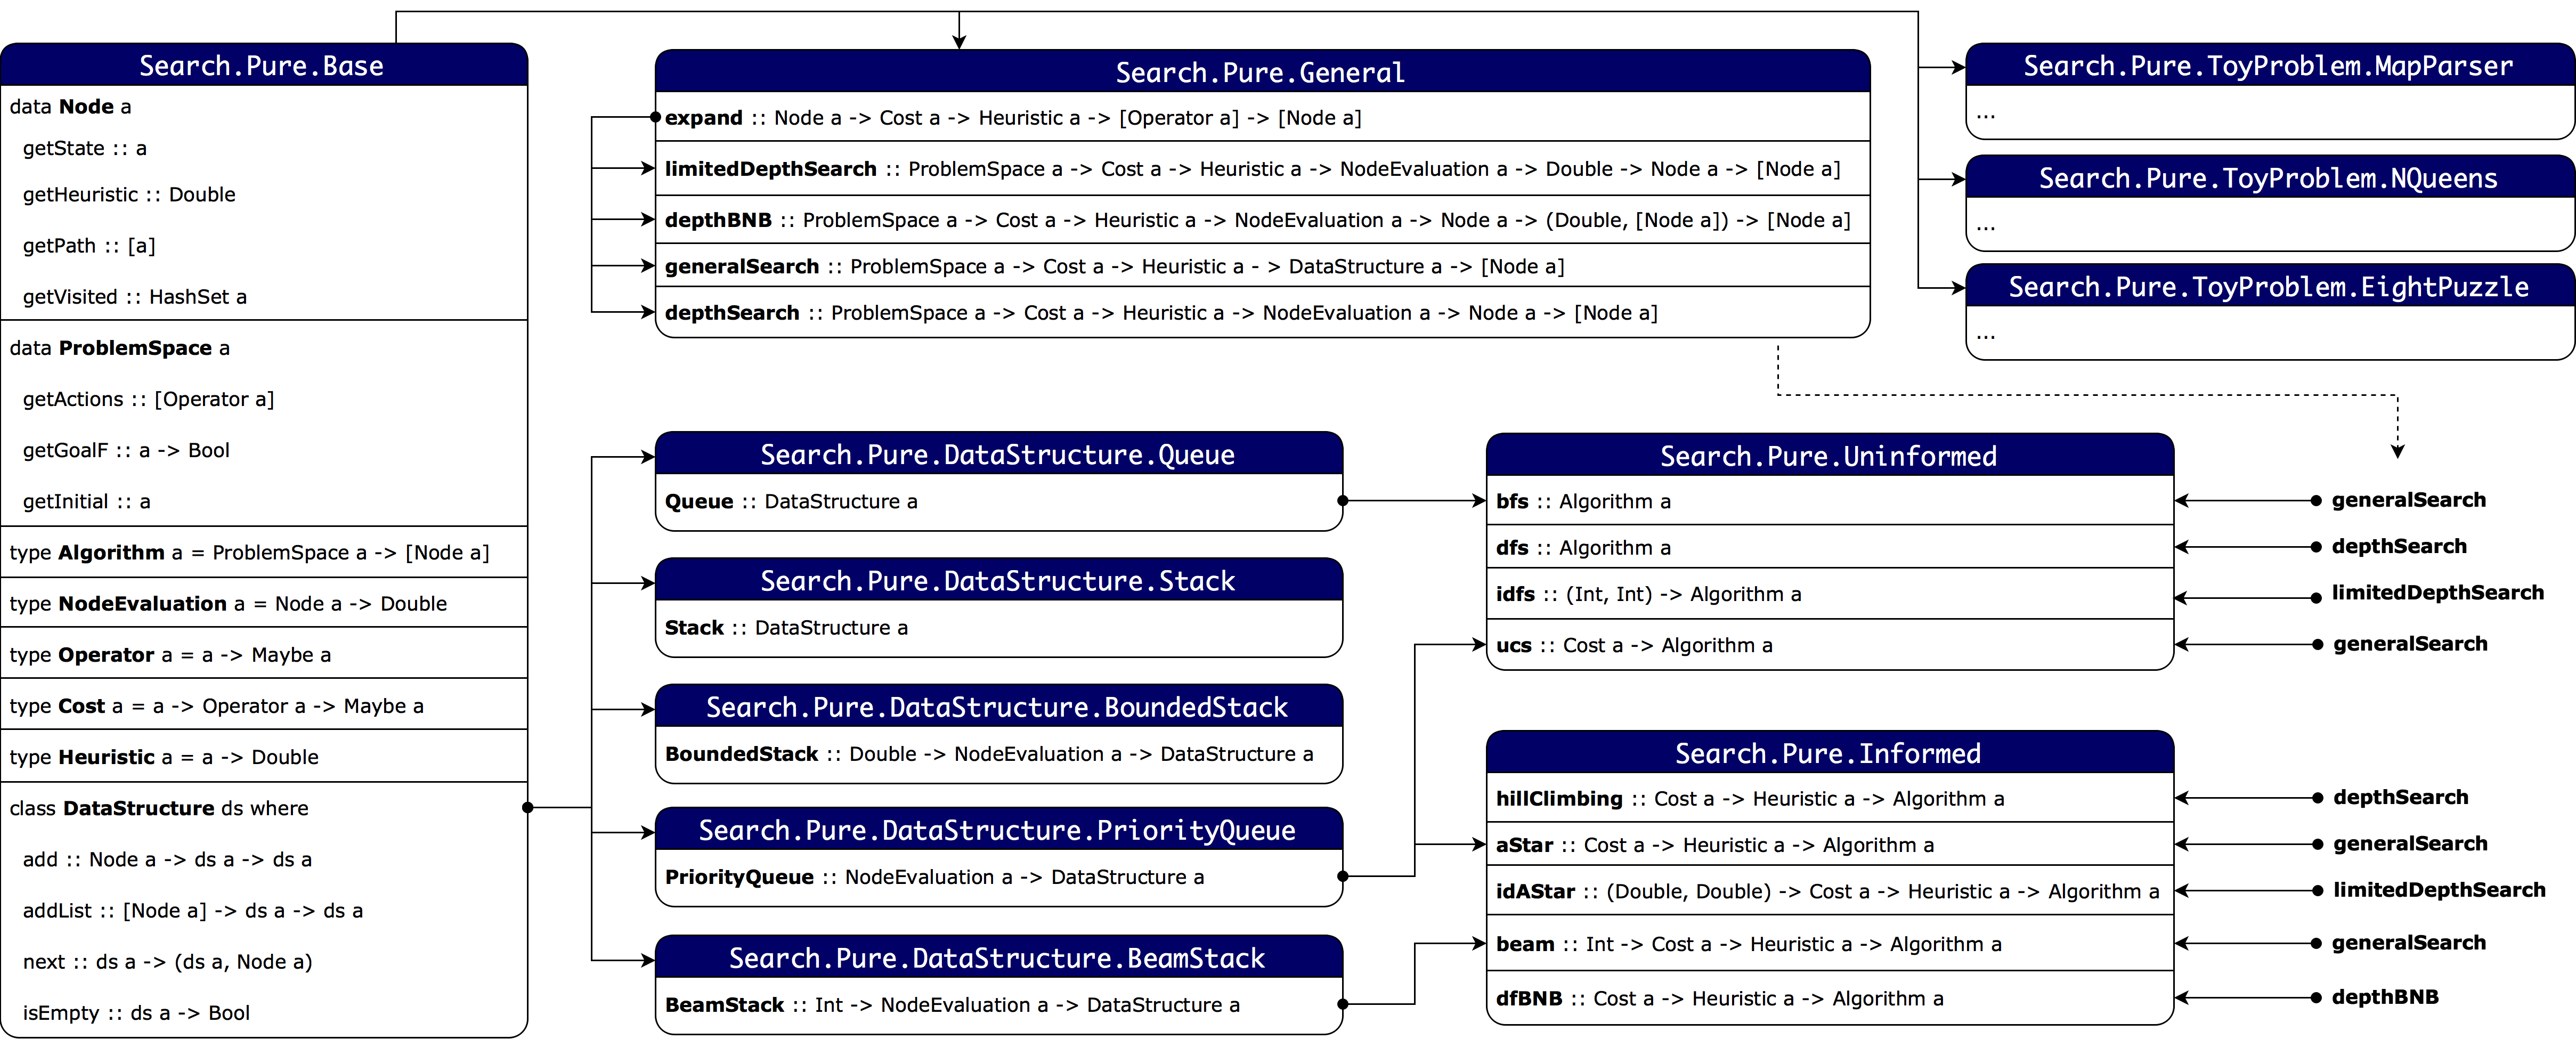
\includegraphics[width=0.9\textwidth]{img/type-graph-pure.png}
  \vspace{1cm}
  \caption{Type signature graph of the \texttt{Search.Pure} library}
  \label{graph-pure}
\end{sidewaysfigure}

\begin{sidewaysfigure}
  \centering
  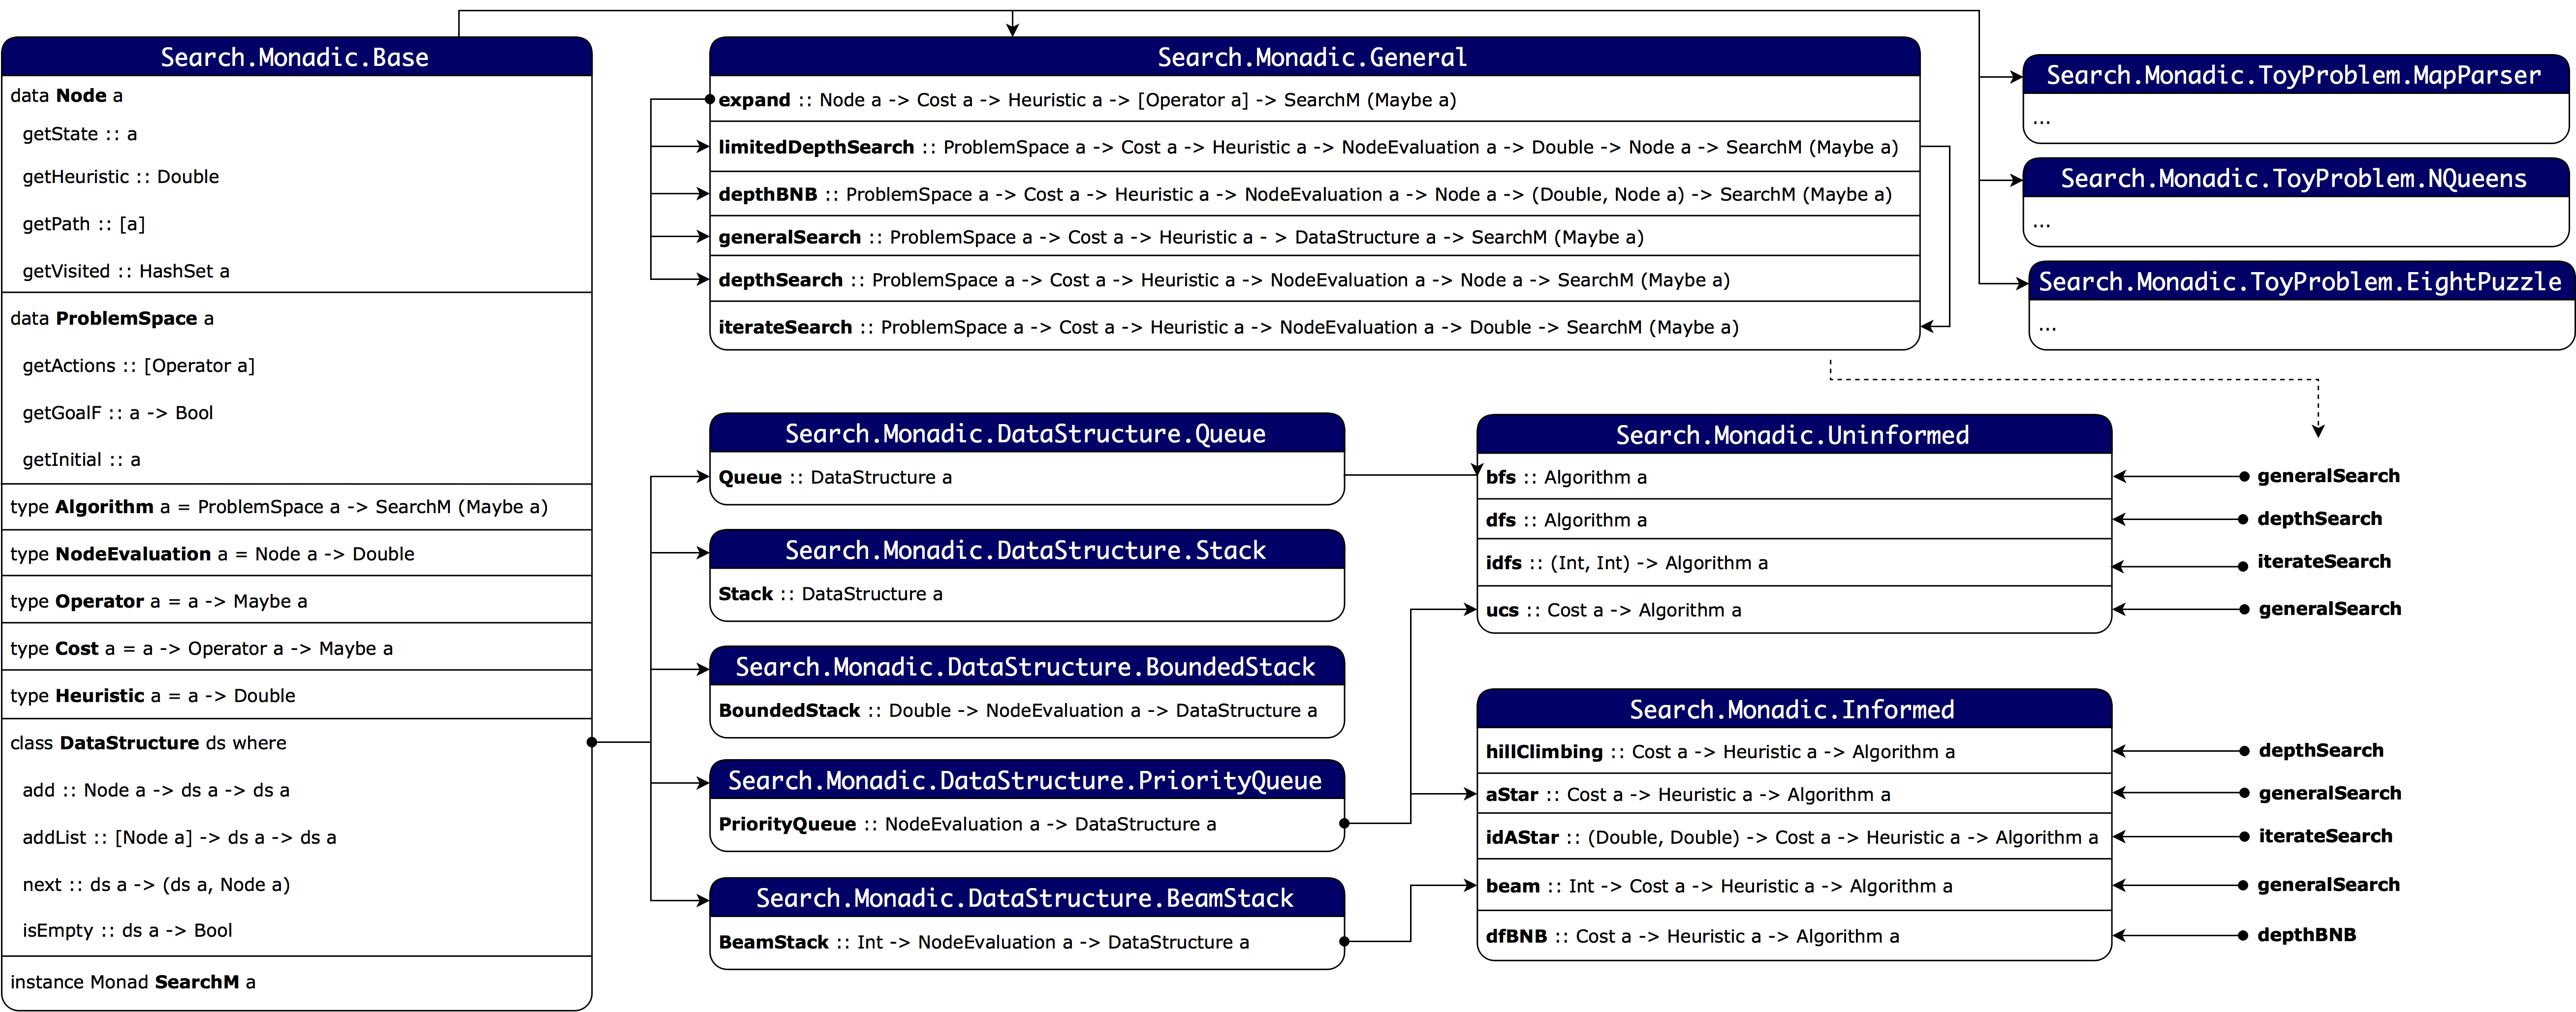
\includegraphics[width=0.9\textwidth]{img/type-graph-monadic.png}
  \vspace{1cm}
  \caption{Type signature graph of the \texttt{Search.Monadic} library}
  \label{graph-monadic}
\end{sidewaysfigure}

These graphs (Figures \ref{graph-pure}, \ref{graph-monadic}) show the basic
control and import flow of the library, and are specially useful for
understanding implementation basics and dependencies among functions. As a
special remark, the specific functions provided by the \texttt{ToyProblem}
modules are omitted (due to lack of interest for the rest of the diagram) as
well as the \texttt{Benchmark} tools, and it is important to notice that every
time the generic type \texttt{a} is mentioned has to follow the constraints
\texttt{Eq a} and \texttt{Hashable a}, since it is the type of the state of the
problem space. Such constraints were dropped from the graph for readability
reasons.\\

We can see how both parts of the library share the same main structure: A
\texttt{Base} module that defines all the main types needed, a \texttt{General}
module that defines the more generalized functions to perform the search, a set
of \texttt{DataStructure} implementations and two modules, \texttt{Uninformed}
and \texttt{Informed} that implement a set of (respectively) uninformed and
heuristic algorithms, using the algorithms and data structures defined in the
former modules. For example, the Breadth-First Search algorithm (\texttt{bfs})
is defined using a \texttt{Queue} data structure and initial conditions of a
\texttt{generalSearch}.\\

Even if both parts of the library seem the same, a closer look reveals that the
monad designed to keep track of the search (\texttt{SearchM}) is returned
instead of a list; a fact that is not visible because it is encapsulated in the
\texttt{Algorithm} type. Also, some noticeable differences like the creation of
new functions to keep better track of search statistics are present in the
\texttt{Monadic} part of the library.\\


\subsection{Implementation}

\subsubsection{General Search}

To perform searches like a Breadth-First search, it is needed to enqueue the
nodes in a structure and check in such structure which one is the next one to
be expanded in the search. This general behavior is mainly modified by the
nature of the data structure used to store the nodes: depending on it, we can
use a queue (for Breadth-First Search), a stack (for a Depth-First Search) or
more complex data structures such as a priority queue (for Uniform-Cost Search
or A* Search, for instance). This general search is indeed described in
\cite{rusell-2003-aima} when first explaining search methods. This algorithm
is the main inspiration for the final implementation of the
\texttt{generalSearch} method.\\

\begin{lstlisting}[style=haskell,
caption=Pure \texttt{generalSearch} implementation, label=pure:general]
generalSearch :: (DataStructure ds, Eq a, Hashable a)
  => ProblemSpace a   -- ^ 'ProblemSpace' to be solved
  -> Cost a           -- ^ 'Cost' function to use
  -> Heuristic a      -- ^ 'Heuristic' function to use
  -> ds a             -- ^ 'DataStructure' that manages the node expansion
  -> [Node a]         -- ^ Returns the list of all final nodes (solutions)

generalSearch problem g h nodes
  | isEmpty nodes                   = []
  | getGoalF problem (getState n)   = n : generalSearch problem g h nodes'
  | otherwise                       = generalSearch problem g h ds'
  where (nodes', n) = next nodes
        expanded = expand n g h (getActions problem)
        ds' = addList expanded nodes'
\end{lstlisting}

We can see in Listing \ref{pure:general} how the implementation is
straightforward: To find all the possible paths to obtain a solution, the
function checks if the node is final and enqueues if to the list of solutions,
or expands it and adds the resulting nodes (if any) to the data structure. This
could keep on going until the data structure is completely empty, but it will
just expand as many nodes as strictly necessary to find the solutions the
function is asked for.\\

This way of relying on the data structure makes a super versatile piece of code
out of this implementation, but also makes it extremely hard to formally prove:
a possible way to do so would be to prove that all the nodes are expanded in a
given order (i.e that a Breadth-First Search expands the nodes in a FIFO way),
but that task depends on the data structure's implementation, so it is not
possible to prove the correctness of this implementation for all possible
entries. To make up for this, we the library includes all unit and integration
tests possible to check correct behavior of it and the default data structures
provided in it.\\

\subsubsection{Linear-Memory Search}

With the \texttt{generalSearch} method we could virtually mimic any possible
algorithm's node expansion order, by adding those functionalities to the data
structure: a stack-like structure will expand nodes in a DFS fashion, adding a
limit of depth will result in an IDFS-like behavior, sorting the nodes in a
priority queue would result in a A* Search. However, stating that all these
behaviors would be a valid implementation of the aforementioned algorithms is a
great underestimation of these designs: there are other aspects to analyze of
an algorithm rather than just the node expansion order
\cite{korf-2014-correct}.\\

A specially problematic aspect for our \texttt{generalSearch} method is the
memory usage: the fact of enqueueing the nodes in the data structure makes it
use an exponential memory depending on the branching factor of the search, and
the fact that the objects in Haskell are immutable only makes this worse. This
is acceptable when performing an A* Search (there is no other way for us to
expand the nodes in order than to sort them in a queue with all the nodes to be
expanded) but trying to use a stack as a data structure to perform a
Depth-First Search will also result in it using exponential memory (all the
nodes get enqueued and passed along the structure). This is not acceptable and
we need to implement a different method for it.\\

Fortunately, implementing this linear-memory method is as easy as relying on
one of Haskell's more natural mechanisms: recursive calls in a tree shape.
However, instead of simple depth-first search, we can take advantage of one of
the most widespread abstractions of the language: \texttt{map}. This function
performs a given function on each of the elements of a list. The main advantage
is that this is one of the abstractions that uses concurrency so may result in
a performance improvement under some certain conditions. In our case, we can
define the method \texttt{depthSearch}, whose pure implementation is defined in
the Listing \ref{pure:depth}.\\

\begin{lstlisting}[style=haskell,
caption=Pure \texttt{depthSearch} implementation, label=pure:depth]
depthSearch :: (Eq a, Hashable a)
  => ProblemSpace a   -- ^ 'ProblemSpace' to be solved
  -> Cost a           -- ^ 'Cost' function to use
  -> Heuristic a      -- ^ 'Heuristic' function to use
  -> NodeEvaluation a -- ^ 'NodeEvaluation' to sort the expanded nodes
  -> Node a           -- ^ Current 'Node' to be expanded
  -> [Node a]         -- ^ Returns the list of all final nodes (solutions)
  
depthSearch problem g h f node
  | getGoalF problem (getState node) = return node
  | otherwise = concatMap (depthSearch problem g h f) sorted
    where sorted = sortBy (\n n' -> compare (f n) (f n')) expanded
          expanded = expand node g h (getActions problem)
\end{lstlisting}

We can see that this implementation includes some interesting mechanics. The
function performs 3 basic tasks: check if a given node contains a final state
inside and leave it, expand non-final nodes and flatten the list. When
flattening the list, the nodes that result in an empty list (that is, that
cannot be expanded) are pruned from the solutions list. By using this, we don't
rely on a sequential implementation and we can take advantage of the
paradigm: this mapping of nodes are actually done concurrently and can increase
the performance compared to a simple recursive call. Also notice that the
function accepts a \texttt{NodeEvaluation} function to sort the nodes. Although
this is not explicitly used in any of the predefined algorithms, can be useful
for an user to sort nodes in order to be expanded.\\

%%% TODO: Diagram explaining work?

However, it is important to note that due to the fact that the each nodes
include in themselves information of their path (the key part to solve the k
path-finding problem) makes the size of the nodes slightly increase as the
search increases. For that reason, the memory is not strictly linear, but it
still provides a huge advantage over the previous method discussed. Since the
memory used is not linear due to the allocation but to the increasing size of
the nodes, this solution will be accepted as good enough for this purpose.\\

This method can be easily modified to perform another type of useful and
widespread linear-memory search: a limited memory search (of any given bound by
the user), that expand nodes if possible or if a given \texttt{NodeEvaluation}
is within the bound given by the user. This function can be read in Listing
\ref{pure:limit}.\\

\begin{lstlisting}[style=haskell,
caption=Pure \texttt{limitedDepthSearch} implementation, label=pure:limit]
limitedDepthSearch :: (Eq a, Hashable a)
  => ProblemSpace a   -- ^ 'ProblemSpace' to be solved
  -> Cost a           -- ^ 'Cost' function to use
  -> Heuristic a      -- ^ 'Heuristic' function to use
  -> NodeEvaluation a -- ^ 'NodeEvaluation' to sort the expanded nodes
  -> Double           -- ^ Limit to be imposed to the 'NodeEvaluation'
  -> Node a           -- ^ Current 'Node' to be expanded
  -> [Node a]         -- ^ Returns the list of all final nodes (solutions)

limitedDepthSearch problem g h f l node
  | getGoalF problem (getState node) = return node
  | otherwise = concatMap (limitedDepthSearch problem g h f l) sorted
    where sorted = sortBy (\n n' -> compare (f n) (f n')) expanded
          expanded = filter ((<l) . f) $ expand node g h (getActions problem)
\end{lstlisting}

With this function, we can implement different search algorithms like
Iterative Depth-First Search or Iterative Deepening A* Search, by performing
a bounded search and increasing the bound over and over.\\

\subsubsection{Branch \& Bound Search}

The last well known general search algorithm that we can provide is a
branch-and-bound fashion search: performing a depth-first search and using the
cost of that solution as the current cost bound. Then, keep on expanding nodes
but making that search be a limited one, by the bound we have found in the
previous solution. Each time a new solution is found, update the bound and keep
on the search until there are no more nodes to expand. This algorithm also uses
linear-space to perform the search, and a pseudocode for it can be found in
\cite{zhang-1995-bnb} along with all necessary explanations.\\

However, this pseudocode is explicitly imperative and seems hard to recreate
using a purely functional approach. A naive approach to this matter would be to
use the previously mentioned algorithms to solve this problem: perform a
\texttt{depthSearch} and store the cost, then perform a
\texttt{limitedDepthSearch} with the current bound and try to found a better
one, and repeat this procedure until no new solution is found. However, this
will not use linear space: instead, it will perform $n$ searches that will,
indeed, use linear-memory each one. This solution is definitely
non-acceptable.\\

The best solution, is to use a fold method, and use such accumulator to hold
both the list of solutions (in a Last In, First Out order) and the current best
cost. Using this fold and recursively calling the function on the nodes, we can
replicate the exact behavior of the algorithm in a purely functional way in a
single search. The code of this function is written in the Listing
\ref{pure:bnb}.\\

\begin{lstlisting}[style=haskell,
caption=Pure \texttt{depthBNB} implementation, label=pure:bnb]
depthBNB :: (Eq a, Hashable a)
  => ProblemSpace a   -- ^ 'ProblemSpace' to be solved
  -> Cost a           -- ^ 'Cost' function to use
  -> Heuristic a      -- ^ 'Heuristic' function to use
  -> NodeEvaluation a -- ^ 'NodeEvaluation' to sort and bound expanded nodes
  -> Node a           -- ^ Current 'Node' to be expanded
  -> (Double, [Node a])    -- ^ The current bound and intermediate solutions
                           -- found (in ascending cost order)
  -> (Double, [Node a])    -- ^ The final bound and all solutions found (in
                           -- ascending cost order)

depthBNB problem g h f n (l, sol) = foldl bnbStep (l, sol) sorted
  where sorted = sortBy (\n n' -> compare (f n) (f n')) expanded
        expanded = expand n g h (getActions problem)

        bnbStep (bound, solutions) n
          | f n >= bound = (bound, solutions)
          | getGoalF problem (getState n) = (f n, n:solutions)
          | otherwise = depthBNB problem g h f n (bound, solutions)
\end{lstlisting}


\subsubsection{Uninformed Algorithms}

Using the previously developed methods, we are able to create a set of
uninformed, purely-functional algorithms ready to use by the users. These
algorithms are just partially-applied general functions which are imposed some
initial conditions to behave as the algorithm is supposed to. Apart from the
convenience that this implies, another main reason to design the search
algorithms this way is because those general search methods are available for
users to build their own search algorithms. Just like these partially-applied
functions result in one algorithm or the other, the users of the framework have
absolute freedom to use them to create their own algorithms.\\

\begin{lstlisting}[style=haskell,
caption=Pure uninformed search algorithms, label=pure:uninf]
-- | 'bfs' runs a Breadth-First Search
bfs :: (Eq a, Hashable a) => Algorithm a
bfs problem = generalSearch problem noCost noHeuristic (startQueue $
                                                        getInitial problem)


-- | 'dfs' runs a Depth-First Search
dfs :: (Eq a, Hashable a) => Algorithm a
dfs problem = depthSearch problem noCost noHeuristic noSorting initial
  where initial = newNode (getInitial problem)


-- | 'idfs' runs an Iterative Deepening Depth-First Search. The first argument,
-- a pair of 'Int's (@step@, @inf@), represent the main parameters of the
-- search: each new iteration the depth test is incremented by adding @step@ as
-- long as the new depth is lower than @inf@.
idfs :: (Eq a, Hashable a) => (Int, Int) -> Algorithm a
idfs (step, inf) p = stepIDFS 0
  where stepIDFS d = if d < inf
          then limitedDepthSearch p noCost noHeuristic depth (fromIntegral d) i
               ++ stepIDFS (d + step)
          else []
        i = newNode $ getInitial p
        depth = fromIntegral . length . getPath


-- | 'ucs' runs an Uniform-Cost Search with a given cost function
ucs :: (Eq a, Hashable a) => Cost a -> Algorithm a
ucs g problem = generalSearch problem g noHeuristic sortedCost
  where sortedCost = startPriorityQueue (getInitial problem) getCost
\end{lstlisting}

In the Listing \ref{pure:uninf} we can see some of the best know brute-force
search algorithms. Breadth-First Search is implemented using a
\texttt{generalSearch} call with a queue data structure (First In, First Out).
On the other hand, the Depth-First Search algorithm uses the simplest
implementation of the \texttt{depthSearch} general method starting in the
initial node of the problem space. Iterative Deepening Depth-First Search is
implemented by performing a \texttt{limitedDepthSearch} over and over,
increasing the depth bound using a given step until that bound is bigger that
some limit given by the user. All these algorithms have been implemented
following the description provided in \cite{rusell-2003-aima}. The last
algorithm in the set is Uniform-Cost Search, which performs a breadth-first,
cost-based search in the problem space. To do so, \texttt{generalSearch} is
used with a priority queue that sorts the nodes in cost ascending order. This
algorithm is usually called Dijkstra's, but this implementation is based on the
description given in \cite{rusell-2003-aima} and due to the nature of the
framework and the language it follows all the criteria exposed in
\cite{felner-2011-dijkstra} to be named Uniform-Cost Search: it works in
implicit graphs (as most all \texttt{ProblemSpace} objects are exactly that),
and Dijkstra's would require to have all nodes input in the $Q$ list.\\


\subsubsection{Informed Algorithms}

In a similar way, we define a set of informed algorithms. The code for these
algorithms can be found in Listing \ref{pure:inf}


\begin{lstlisting}[style=haskell, caption=Pure informed search algorithms,
label=pure:inf]
-- | 'hillClimbing' runs a Hill Climbing Heuristic Search.
hillClimbing :: (Eq a, Hashable a) => Cost a -> Heuristic a -> Algorithm a
hillClimbing g h problem = generalSearch problem g h sortedH
  where sortedH = startPriorityQueue (getInitial problem) getHeuristic


-- | 'aStar' runs an A* Search.
aStar :: (Eq a, Hashable a) => Cost a -> Heuristic a -> Algorithm a
aStar g h problem = generalSearch problem g h sortedAStar
  where sortedAStar  = startPriorityQueue (getInitial problem) aStarF
        aStarF n = getCost n + getHeuristic n


-- | 'idAStar' runs an Iterative-Deepening A* Search.
idAStar :: (Eq a, Hashable a) =>
  (Double, Double) -> Cost a -> Heuristic a -> Algorithm a
idAStar (step, inf) g h p = stepIDAStar 0
  where stepIDAStar l = if l < inf
          then limitedDepthSearch p g h aStarF l initial
               ++ stepIDAStar (l + step)
          else []
        aStarF n = getCost n + getHeuristic n
        initial = newNode (getInitial p)


-- | 'beam' runs a Beam Search of a given beam width.
beam :: (Eq a, Hashable a) =>
  Int -> Cost a -> Heuristic a -> Algorithm a
beam w g h problem = generalSearch problem g h stack
  where stack = startBeamStack (getInitial problem) w getHeuristic


-- | 'dfBNB' performs a Depth-First Branch & Bound Search. Due to the nature of
-- this algorithm, it does not return the list of all solutions in the problem
-- space: Instead, it returns all the solutions that it has found in ascending
-- cost order.
dfBNB :: (Eq a, Hashable a) =>  Cost a -> Heuristic a -> Algorithm a
dfBNB g h problem = snd $ depthBNB problem g h aStarF initial (inf, [])
  where aStarF n = getCost n + getHeuristic n
        initial = (newNode . getInitial) problem
        inf = 1/0
\end{lstlisting}


The first of them is a greedy heuristic search algorithm, better known under
the name of Hill Climbing. This algorithm performs a \texttt{generalSearch}
with a priority queue that sorts the nodes in ascending order of heuristic
value. Arguably, the most popular informed search algorithm, A* Search, is
implemented in a similar way: runs a \texttt{generalSearch} using a priority
queue as well, but that priority queue uses a function $f(n) = g(n) +
h(n)$ to sort the nodes in ascending order, where $g$ is the cost function and
$h$ is the heuristic function. A more lightweight but similar algorithm is
Iterative-Deepening A*, which performs a depth search using the aforementioned
function under a certain bound that increases each new iteration. This searches
take linear time to find the solution, and if IDS performs a search inside a
certain depth, IDA* performs a search inside a certain $f$-spectrum.

\newpage

%%% Local Variables:
%%% TeX-master: "tfg"
%%% End: